\section{Design}
\label{sec:design}

\begin{figure}[ht]
\begin{centering}
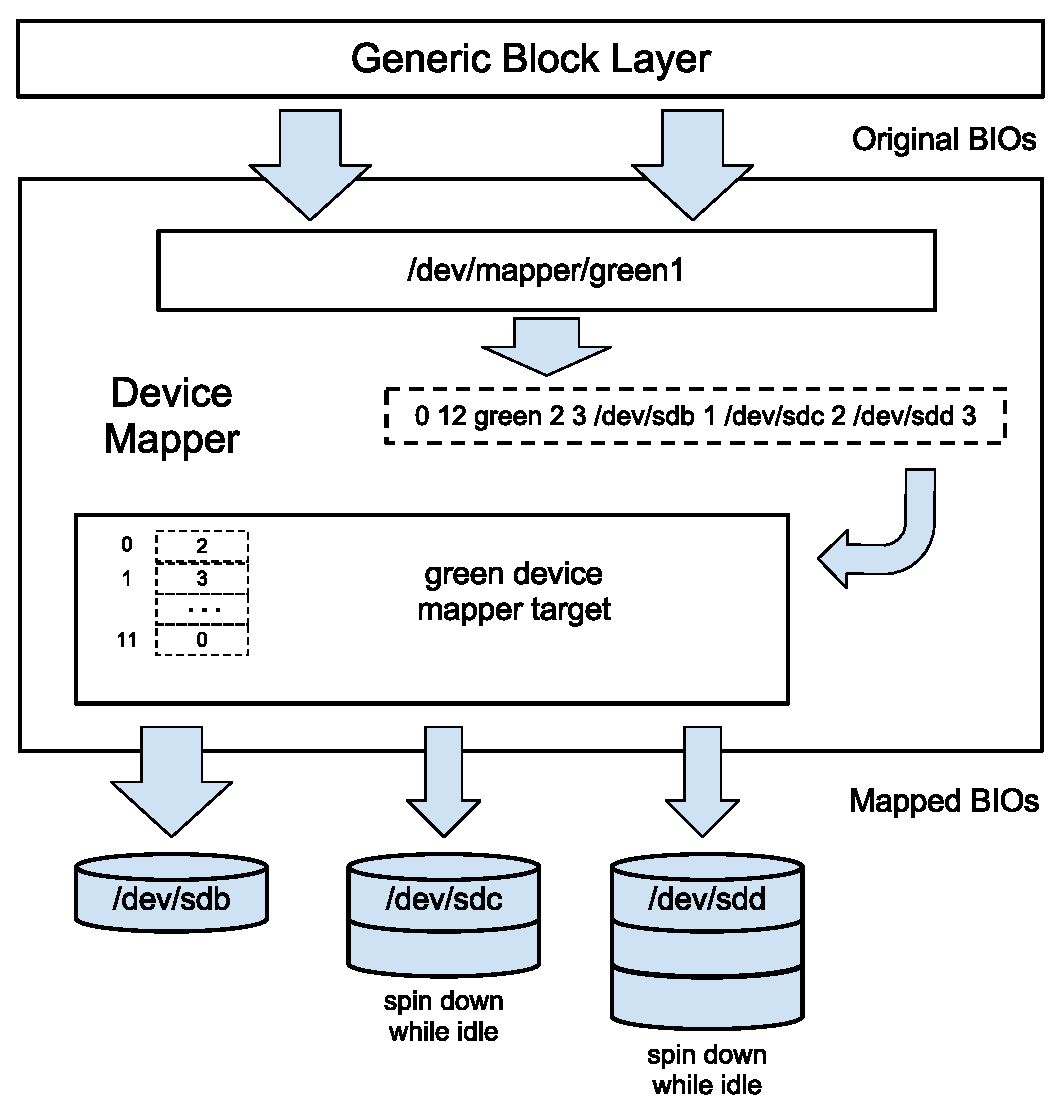
\epsfig{file=figures/dm.eps,width=1.00\linewidth}
\caption{Linux Device Mapper and Green Device Mapper Target.
'/dev/mapper/green1' is a created virtual block device. The two dashed
boxes are mapping tables. The first one is used by Device Mapper to
delegate mapping to target; the second one is used internally by the
green target.}
\label{fig:dm}
\end{centering}
\end{figure}

We present the design of our green multi-disk driver as a Linux Device
Mapper target. Linux Device Mapper, as depicted in Figure
\ref{fig:dm}, is a generic framework to map one block device onto
another. It works by processing data passed in from a virtual block
device, that it itself provides, and then passing the resultant data
on to another block device \cite{wiki_dm}. The advantage of Device
Mapper is that it can provide virtual devices to user programs and
kernel modules above block level without exposing details of
underlying devices. Thanks to this transparency, the underlying
devices can be of different size and type (can in turn be virtual or
physical) and the mapping can be performed in different manners. As
essentially a middle-ware sitting between the Generic Block Layer and
block devices. Device Mapper receives BIOs, which is a kernel
structure describe I/O requests, from Generic Block Layer, then
redirect them to other block devices by modifying the target device
and sector offset. 

Device Mapper itself does not perform the redirection. It delegates
this operation to Device Mapper targets, which are registered kernel
modules performing certain kinds of mapping. This delegation is
specified in a mapping table, which contains the type of responsible
Device Mapper target for certain regions of block devices. In Figure
\ref{fig:dm}, all I/O request to sectors [0, 0+12) of virtual device
"/dev/mapping/green1" will be handled by a target named green; all
parameters after "green" are passed to the green target. A mapping
target contains functions to construct/destruct mapped devices, map
I/O requests, merge adjacent I/O requests, report and control device
status.

\subsection{Design Goals}
The design goal of our green multi-disk Device Mapper target is driven
by the following guiding principles: 

\begin{itemize}

\item \textbf{Save energy by allowing disks to spin/power down}. Be
energy efficiency is one of the most important features our green
multi-disk target is pursuing. The SSD cache benefits both I/O
performance and energy efficiency simultaneously. In this study, we
are more concerned of the latter. We have made trade-offs between
energy efficiency and other desirable features such as capacity.

\item \textbf{Use SSD aware data structures and algorithms}. While SSD
provides better I/O performance and energy efficiency, it has its own
constraints including limited erase-write cycles and inefficient
random writes. This principle guides our design to avoid these
constraints and extract maximum benefit out of SSD.

\item \textbf{Provide stable and robust storage}. Because our green
target provides customized block mapping and data grouping, it is
critical to always perform correct translation from virtual to
physical blocks. It should not lose mapping information in case of
power failure or other hazardous incidents.

\end{itemize}

\subsection{Disk Management}

Device Mapper targets maintain mapping of sectors between virtual and
physical disks. The straightforward method is to maintain a
sector-wise mapping table. However, it is prohibitive because its size
is too large to fit in memory. For example, the size of sector-wise
mapping table of a 1TB disk (512-byte sectors) is as large as 8GB with
4-bytes table entries. Store the mapping table on disk (even on SSD)
is not an option because it is too slow to incur extra I/O. A solution
is to divide disks into larger units. Here, we adopt the LVM term
extent, which is the unit of disk managed by LVM, typically 4MB. Then
the mapping becomes extent-wise and its size diminishes to 1MB in the
above example. 

In our green target, multiple physical disks are mapped as a single
virtual disk. The physical disks are linearly organized in the order
of energy efficiency, i.e., the most energy-efficient one goes first
and so on. In Figure \ref{fig:dm}, '/dev/sdb' is the most
energy-efficient one but with smallest capacity, i.e., SSD; '/dev/sdc'
and '/dev/sdd' follow decreasingly in energy efficiency and
increasingly in capacity. This makes the addressing of physical
sectors easy. An extent index and an offset within extent would
suffice. We have noticed the case that one I/O request on logically
sequential blocks might be mapped to multiple I/O requests on
physically non-sequential blocks. Namely, the translation is performed
per extent instead of per request. However, extent is of big size, so
it is unlikely that the extent by extent translation becomes a
performance bottleneck. Furthermore, the Device Mapper framework
provides interface to merge adjacent I/O requests, which also
alleviate this problem.

The exact size of extent is an important factor as it affects not only
memory consumption but also granularity of mapping and data migration.
A large size of extent has the following impacts: 

\begin{itemize} 

\item \textbf{Smaller mapping table}. As already discussed, the
adoption of extent makes the mapping table becomes extent-wise and
small. 

\item \textbf{More aggressive pre-fetch}. As energy-efficient disk such
as SSD have similar effect as disk cache. When a large extent of data
is moved onto SSD, it can be consider as an aggressive pre-fetch. 

\item \textbf{Coarse-grain data migration among disks and more
sequential I/O}. Because the major latency of magnetic disk is seek
time, a larger sequential migration will not significantly slow down
the I/O. Moreover, with large size of migration unit, there are fewer
I/O because adjacent sectors are processed in batch. This is beneficial
to the life time of SSD as well considering its limited erase-write
cycles.

\item \textbf{High overhead}. Since each extent can represent several
sectors, more sectors I/O can be wasted in case of wrong prediction
thus adds overhead to the overall system. 

\end{itemize}

Physical extents are managed using a bitmap. The extents on SSD are
taken specially. Besides recorded in the bitmap, they are also linked
in two lists, one for free extents and the other for used. This
facilitates and speeds up manipulation of the extents on SSD, which
happens very frequently.

Different workloads might favor different extent sizes depending on
file sizes, I/O frequency and read-write ratio. Therefore, we make
extent size a configurable parameter to the green target so that
different trade-offs can be made via configuration. 

%-----------------------------------------------------------------------------

\subsection{Mapping Table}

There are two mapping tables in Figure \ref{fig:dm}. One is actually a
configuration file used by the Device Mapper framework; the other
contains extent-wise mapping information used internally by our green
target. We are talking about the second one in following discussion. 

The straightforward structure of the mapping table is an array of the
size of extent number on all physical disks. The mapping table is
maintained in memory and can be cached, so its lookup is fast. Besides
mapping information, the table also contains other fields including
flags, timestamp of the latest access and number of total access
(possibly distinguished read from write). Flags are used to record
states of extents, which include, for example, 1) whether the extent
is accessed or not recently; 2) whether the extent is under migration
or not; and 3) whether the extent is updated or not when it is under
migration. Timestamp of the latest access and number of total access
are used to predict hot extent. 

The mapping table need be saved onto disk on power off as metadata. To
be fail-safe, it has a replicate in every physical disk. The in-memory
version and on-disk version of mapping table can be slightly
different, since it is not necessary to save online information such
as timestamp of latest access. To be robust in case of hazardous
situation such as power failure, the mapping table is flushed onto
disk periodically. To prevent this periodical background job from
disturbing other disks' idle periods, this flush saves the table only
on the cache disk. Table on other disks are only updated on request or
when the system is being shutting down.

%-----------------------------------------------------------------------------

\subsection{Extent Migration}

There are two kinds of data migration. The first is moving an extent
into the SSD disk, called promotion. The second is moving an extent
out of it, called demotion (similar to eviction in cache management).
Both of them are achieved using kcopyd, the infrastructure of the Device
Mapper framework for copying data between disks. 

Promotion occurs when an extent on secondary disks becomes hot and
there is free extents on SSD. To predict hot extent, we adopt a greedy
approach and take the extent just been accessed as hot. However, a
trade-off between I/O performance and SSD life time is possible when
performing promotion of an extent being written. Because SSD has
limited erase-write cycles, it makes sense to directly map writes to
secondary disk instead of promoting the extent at once. If that extent
is read immediately, then we promote it. This will be helpful in case
of operations like file copying and file appending, wherein disk is
written just once. This does not have significant influence on energy
efficiency because the secondary disk hosting that extent has to spin
up no matter we promote it right now or not. Once it is up, there is a
relative long timeout before it can spin down again because of the
large penalty (latency and short disk life time) of disk spin-down,
so no additional spin-up is needed if that extent is read soon.
Actually, there is research trying to extend SSD lifetime by using HDD
as write cache \cite{hddcache}. However, this is a configurable
feature that allows user to make informed decision when workload
knowledge is available. 

Demotion occurs when the number of free prime extents falls below a
minimum threshold. Demotion tries to evict cold extents on SSD until
the number of free extents goes up to a maximum threshold. There is a
daemon running in background to keep the number of free extents
between the minimum and maximum thresholds. The minimum threshold is
used to ensure that free extents can be readily obtained when
promotions are needed. The maximum threshold is used to demote extents
in batch so that secondary disks are disturbed less. However, these
two thresholds are also parameters that can be changed. When both of
them are 1, the demotion becomes just like cache eviction. To find
cold extent on SSD, a LRU algorithm is used.

\subsection{Data Grouping}

We have studied the data grouping in \cite{Wildani_grouping}. However,
right now, very little thing about data grouping has been done in our
implementation. A simple heuristic we are going to experiment is to
group data by frequency of access. That is, most accessed data are all
mapped on to the first disk, namely, SSD and so forth. The reason
behind this is that it is likely for data in same working set to
exhibit access frequency at same level. 

%%%%%%%%%%%%%%%%%%%%%%%%%%%%%%%%%%%%%%%%%%%%%%%%%%%%%%%%%%%%%%%%%%%%%%%%%%%%%%
%% For Emacs:
% Local variables:
% fill-column: 70
% End:
%%%%%%%%%%%%%%%%%%%%%%%%%%%%%%%%%%%%%%%%%%%%%%%%%%%%%%%%%%%%%%%%%%%%%%%%%%%%%%
%% For Vim:
% vim:textwidth=70
%%%%%%%%%%%%%%%%%%%%%%%%%%%%%%%%%%%%%%%%%%%%%%%%%%%%%%%%%%%%%%%%%%%%%%%%%%%%%%
% LocalWords:  
